Pour réduire sa facture d'électricité, Camille a décidé de faire poser des panneaux solaires sur le toit de sa maison.

Elle souhaite analyser sa production et estimer le temps nécessaire pour rentabiliser cet investissement.

\textbf{Les deux parties suivantes sont indépendantes.}

\subsection*{Partie A}

Lors d'une belle journée ensoleillée, la puissance électrique en kilowatt (kW) des panneaux solaires de Camille peut être modélisée en fonction de l'heure par une fonction $f$. On admet que $f$ est définie sur $[0 ; 24]$ et on donne sa courbe représentative $\mathcal{C}_{f}$ ci-dessous.

Avec la précision permise par le graphique :

\begin{center}
	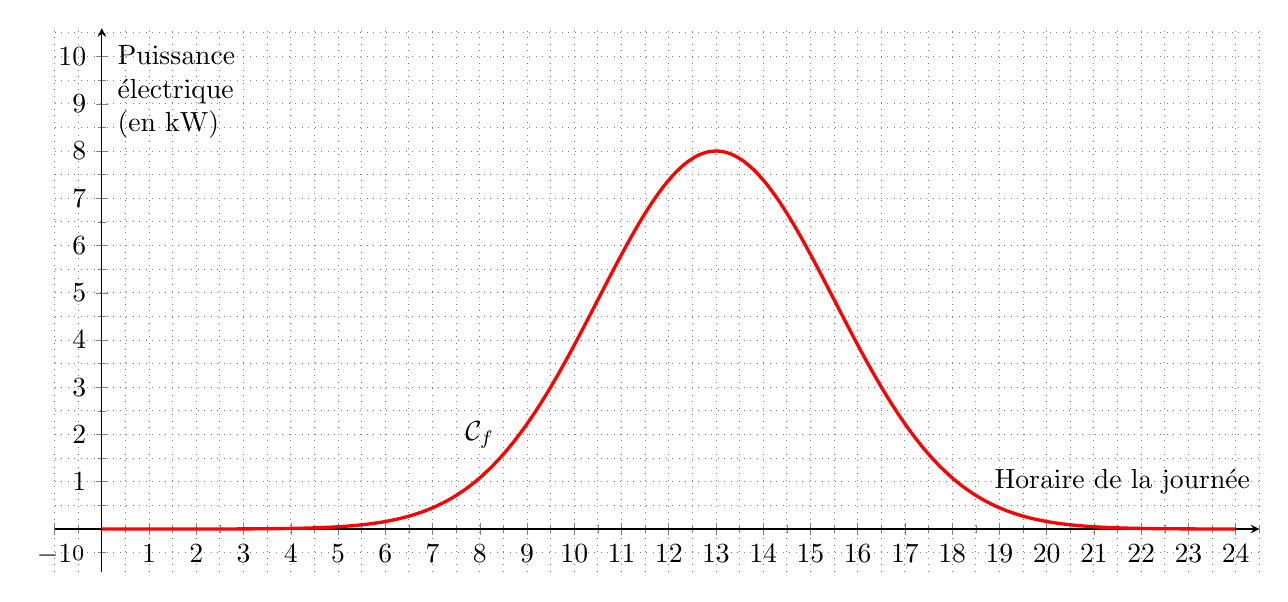
\begin{tikzpicture}
		\begin{axis}[/pgf/number format/.cd, use comma,
			x={6mm}, y={6mm},
			xmin = -1, xmax = 24.5,
			ymin = -0.9, ymax = 10.6,
			xtick distance=1,
			ytick distance=1,
			minor tick num = 1,
			grid=both, axis lines =center,
			grid style={gray!,line width=0.35pt,dotted}]
			\addplot[line width=1.2pt,color=red,smooth,samples=100,domain= 0:24] {8*exp(-0.08*(x-13)*(x-13))};
			\node[below left=1mm] at (axis cs: 0,0) {{\footnotesize 0}};
			\node at(axis cs: 8,2) {$ \mathcal{C}_f $};
			\node[text width=2cm] at(axis cs: 2,9.25) {Puissance électrique (en kW)};
			\node at(axis cs: 21.6,1) {Horaire de la journée};
		\end{axis}
	\end{tikzpicture}
\end{center}















\begin{enumerate}
	\item Donner la puissance électrique des panneaux solaires à 11 h 00.

	\item Résoudre graphiquement l'inéquation \quad $f(x) \geqslant 5$ \quad et interpréter ce résultat dans le contexte de l'énoncé.
\end{enumerate}

\subsection*{Partie B}
Le coût pour 1 kilowattheure (kWh) consommé au tarif réglementé était de 0,15~\euro{} en 2020. On admet que ce tarif réglementé augmente de 6~\% chaque année.

On note $c_{n}$ le coût en euros (\euro{}) pour 1 kWh consommé durant l'année $2020+n$, avec $n$ un entier naturel. On a alors $c_{0}=0,15$.

\begin{enumerate}
	\item Déterminer la nature de la suite $\left(c_{n}\right)$. On précisera sa raison.

	\item Pour tout entier naturel $n$, exprimer $c_{n}$ en fonction de $n$.

	\item Donner le calcul permettant d'obtenir le coût pour 1 kWh consommé en 2030. II n'est pas demandé d'effectuer ce calcul.

	\item On admet que, chaque année depuis 2020, l'utilisation des panneaux solaires de Camille lui a permis d'éviter l'achat de \np[kWh]{2000} par an.
	L'installation des panneaux solaires en janvier 2020 a coûté à Camille 7000~\euro{}.
	On considère le programme Python ci-contre.

	\begin{minipage}{0.5\linewidth}
		\begin{enumerate}
			\item Dans le contexte de l'énoncé, que représentent les variables \texttt{c} et \texttt{S} du programme ?

			\item On exécute le programme ci-contre.

			II affiche 16.

			Interpréter ce résultat dans le contexte de l'énoncé.
		\end{enumerate}
	\end{minipage}
\hfill
\begin{minipage}{0.37\linewidth}
\hfill
\begin{ttfamily}
\begin{tblr}{hline{1,Z}={solid}, vlines,colspec={X},rowsep=0pt}
	n = 0\\
	c = 0.15\\
	S = 0\\
	while S < 7000 :\\
	\qquad S = S + c*2000\\
	\qquad n = n+1\\
	\qquad c = 1.06* c\\
	print(n)\\
\end{tblr}
\end{ttfamily}
\end{minipage}
\hfill~
\end{enumerate}
